%%This is a very basic article template.
%%There is just one section and two subsections.
\documentclass[times,10pt,twocolumn,a4paper]{article}
\usepackage{ncvpripg}
\usepackage{times}
\usepackage[pdftex]{graphicx}	
\usepackage[cmex10]{amsmath}
\usepackage{url}

\title{Stagnant Water Detection Using quadcopter}
\author{}
\def\iccvPaperID{0000}
\begin{document}
\maketitle

\begin{abstract}
Recently, in urban areas there has been a sharp increase in dengue and malaria.
One of the major reason for this is suspected to be the amount of stagnant
water around residencies. There are many areas around urban residential places
such as terraces of high rise buildings, and shades above windows
(\emph{chhajja}) that are hard to reach and hence to inspect. We use quadcopter
to inspect such areas and detect whether there is stagnant water.

\end{abstract}

\section{Introduction}

\subsection{Significance of problem}
\cite{WHO15Malaria} \cite{Cecilia14} \cite{WHO15Dengue} \cite{Microsoft15}

\section{Related Work}

\cite{rankin11}\cite{santana12}\cite{zhang10}

\section{Methodology}

\subsection{SVM classifier}


\begin{figure}[h!]
\centering
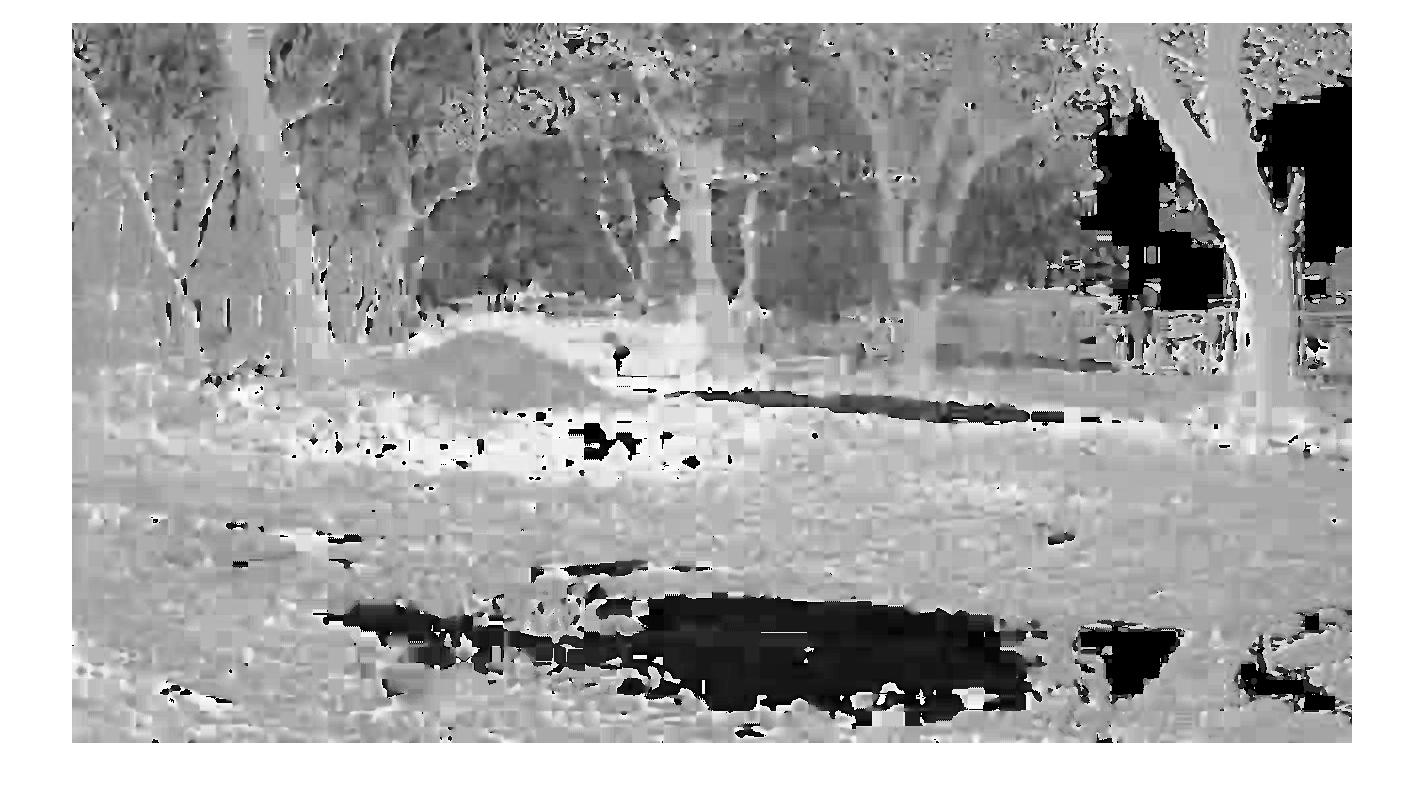
\includegraphics[width=0.3\linewidth]{images/IMG_PAIR_1_1_H.jpg}
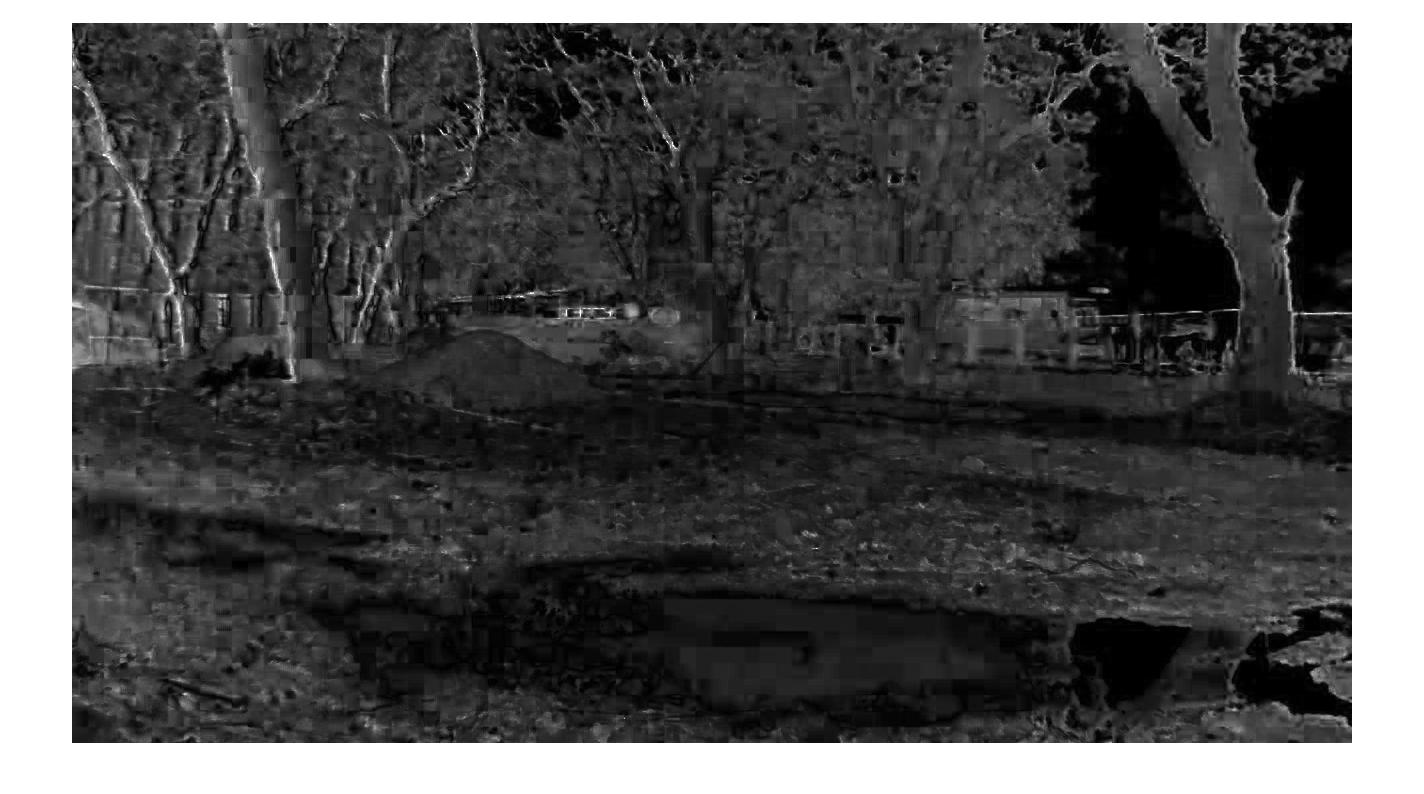
\includegraphics[width=0.3\linewidth]{images/IMG_PAIR_1_1_S.jpg}
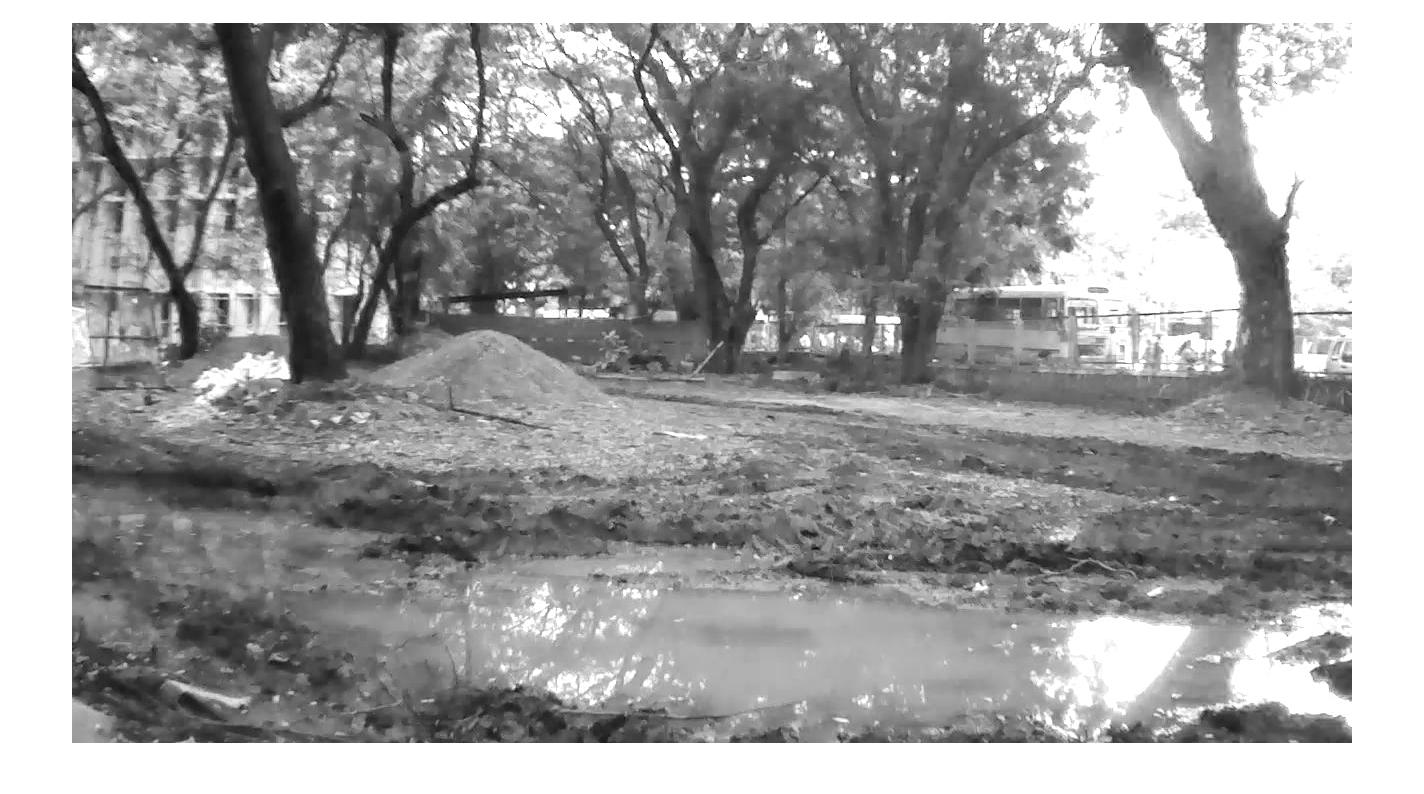
\includegraphics[width=0.3\linewidth]{images/IMG_PAIR_1_1_V.jpg}
\caption{H, S and V of sample image}
\label{fig:HSV}
\end{figure}

\cite{Chapelle99}

\subsection{Optical flow based technique}
\cite{Liu11Thesis}

\cite{Liu11} 
\subsection{Combined approach}

\section{Experiments and Results}
\subsection{Datasets}
\subsection{Creation of training Data}
\subsection{Comparison with prior technique}
\subsection{Quantitative analysis}
\section{Comclusion and Future Work}

\bibliographystyle{IEEEtran}
\bibliography{egbib}
\end{document}
